\chapter{Results}

\label{ch:Results}


%
%
%
%
%
\section{Architectures}

\begin{itemize}
\item $\beta$-VAE used this archiecture 
\item It captured generative factors well
\item Since we know this network can, we use something similar with a 
\item MNIST, Frey, Pong, Space Invaders and Breakout
\item We wish to be able to achieve a similar result with altering activations of specific filters
\end{itemize}


\begin{table}[]
\centering
\label{my-label}
\begin{tabular}{@{}lll@{}}
\toprule
\textbf{Layer} & \textbf{Output shape} & \textbf{Connected to}  \\ \midrule
InputLayer     & (1, 84, 84)           &                        \\
Conv2D\_1      & (32, 42, 42)          & InputLayer             \\
Conv2D\_2      & (64, 21, 21)          & Conv2D\_1              \\
Conv2D\_3      & (1, 8, 8)             & Conv2D\_2              \\
Conv2D\_4      & (1, 8, 8)             & Conv2D\_2              \\
Sampling       & (1, 8, 8)             & Conv2D\_3 \& Conv2D\_4 \\
Deconv2D\_1    & (64, 20, 20)          & Sampling               \\
Deconv2D\_2    & (32, 40, 40)          & Deconv2D\_1            \\
Deconv2D\_3    & (1, 84, 84)           & Deconv2D\_2           
\end{tabular}
\caption{Fully-convolutional single-filter variational autoencoder.}
\end{table}


\begin{table}[]
\centering
\label{my-label}
\begin{tabular}{@{}lll@{}}
\toprule
\textbf{Layer} & \textbf{Output shape} & \textbf{Connected to}  \\ \midrule
InputLayer     & (1, 84, 84)           &                        \\
Conv2D\_1      & (32, 42, 42)          & InputLayer             \\
Conv2D\_2      & (64, 21, 21)          & Conv2D\_1              \\
Conv2D\_3      & (8, 8, 8)             & Conv2D\_2              \\
Conv2D\_4      & (8, 8, 8)             & Conv2D\_2              \\
Sampling       & (8, 8, 8)             & Conv2D\_3 \& Conv2D\_4 \\
Deconv2D\_1    & (64, 20, 20)          & Sampling               \\
Deconv2D\_2    & (32, 40, 40)          & Deconv2D\_1            \\
Deconv2D\_3    & (1, 84, 84)           & Deconv2D\_2           
\end{tabular}
\caption{Fully-convolutional multi-filter variational autoencoder.}
\end{table}


\begin{table}[]
\centering
\label{my-label}
\begin{tabular}{@{}lll@{}}
\toprule
\textbf{Layer} & \textbf{Output shape} & \textbf{Connected to}  \\ \midrule
InputLayer     & (3, 84, 84)           &                        \\
Conv2D\_1      & (32, 42, 42)          & InputLayer             \\
Conv2D\_2      & (64, 21, 21)          & Conv2D\_1              \\
Conv2D\_3      & (8, 8, 8)             & Conv2D\_2              \\
Conv2D\_4      & (8, 8, 8)             & Conv2D\_2              \\
Sampling       & (8, 8, 8)             & Conv2D\_3 \& Conv2D\_4 \\
Deconv2D\_1    & (64, 20, 20)          & Sampling               \\
Deconv2D\_2    & (32, 40, 40)          & Deconv2D\_1            \\
Deconv2D\_3    & (3, 84, 84)           & Deconv2D\_2           
\end{tabular}
\caption{Fully-convolutional single-filter variational autoencoder for RGB images.}
\end{table}


%
%
%
%
%
\section{Learning Generative Factors in Dense Latent Spaces}

\begin{itemize}
\item Reconstruction 
\item Sampling
\item MNIST, Frey, Pong, Space Invaders and Breakout
\item We wish to be able to achieve a similar result with altering activations of specific filters
\end{itemize}


%
%
%
%
%
\section{Single Latent Filter}

\begin{itemize}
\item Consider two architectures: shallow and deep
\item Consider Pong, Space Invaders (in progress) and Breakout
\item Plot reconstruction loss and KL divergence
\item Show reconstructions and convolutional layers of each
\item Show mean activations of filters
\item Alter latent space variable and show reconstruction
\end{itemize}


\begin{figure*}[h!]
\centering
\captionsetup{justification=centering}
    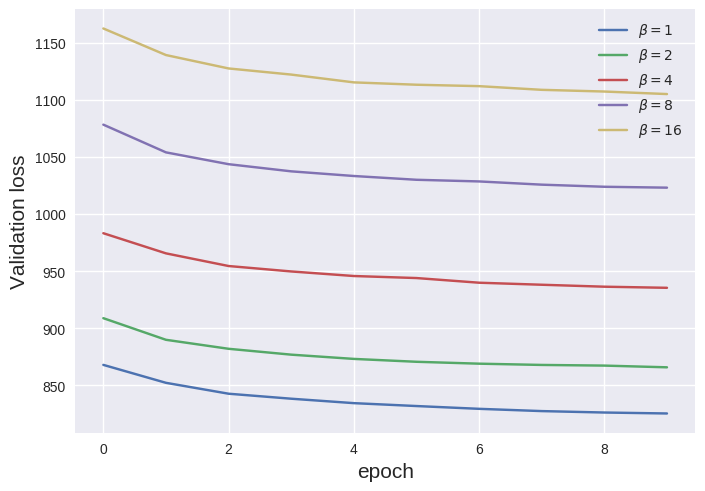
\includegraphics[scale=0.5]{figures/results/latent_image/val_loss.png}
    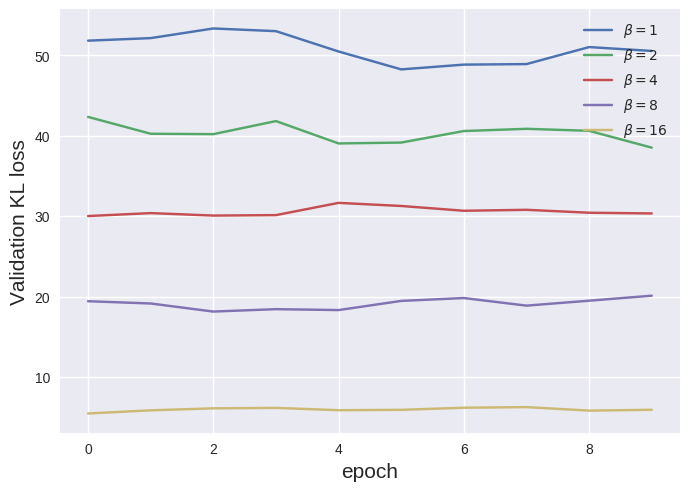
\includegraphics[scale=0.5]{figures/results/latent_image/val_kl_loss.png}
    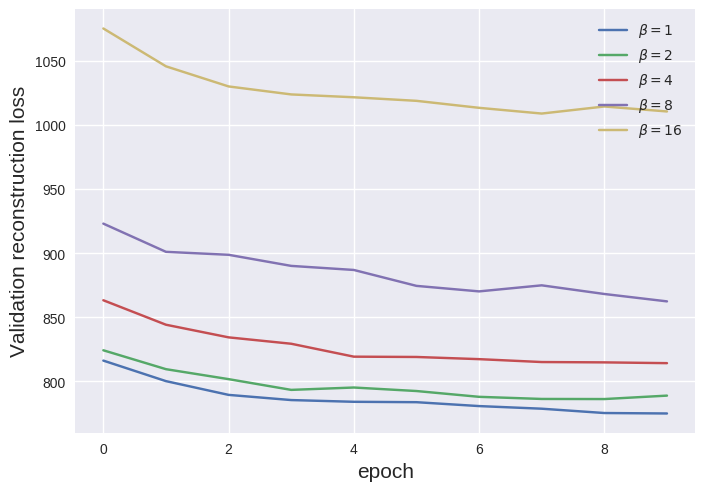
\includegraphics[scale=0.5]{figures/results/latent_image/val_reconstruction_loss.png}
\caption{Latent image.}
\label{fig:latent_image_graphs}
\end{figure*}



\begin{figure*}[h!]
\centering
\captionsetup{justification=centering}
\begin{multicols}{4}
    \includegraphics[scale=0.4]{figures/results/latent_image/beta_1_sample_0_original.png}
    \caption{Original}
    \includegraphics[scale=0.4]{figures/results/latent_image/beta_1_sample_0_reconstructed.png}
    \caption{$\beta = 1$}    
    \includegraphics[scale=0.4]{figures/results/latent_image/beta_2_sample_0_reconstructed.png}
    \caption{$\beta = 2$}
    \includegraphics[scale=0.4]{figures/results/latent_image/beta_4_sample_0_reconstructed.png}
    \caption{$\beta = 4$}
\end{multicols}
\begin{multicols}{4}
    \includegraphics[scale=0.4]{figures/results/latent_image/beta_1_sample_2_original.png}
    \caption{Original}
    \includegraphics[scale=0.4]{figures/results/latent_image/beta_1_sample_2_reconstructed.png}
    \caption{$\beta = 1$}    
    \includegraphics[scale=0.4]{figures/results/latent_image/beta_2_sample_2_reconstructed.png}
    \caption{$\beta = 2$}
    \includegraphics[scale=0.4]{figures/results/latent_image/beta_4_sample_2_reconstructed.png}
    \caption{$\beta = 4$}
\end{multicols}
\begin{multicols}{4}
    \includegraphics[scale=0.4]{figures/results/latent_image/beta_1_sample_3_original.png}
    \caption{Original}
    \includegraphics[scale=0.4]{figures/results/latent_image/beta_1_sample_3_reconstructed.png}
    \caption{$\beta = 1$}    
    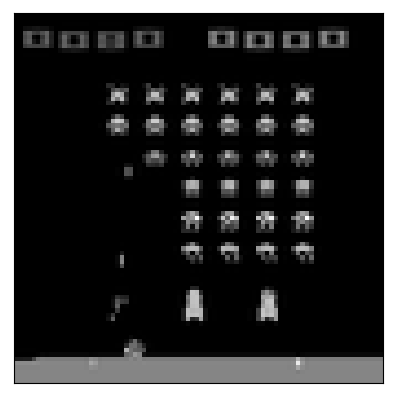
\includegraphics[scale=0.4]{figures/results/latent_image/beta_2_sample_3_reconstructed.png}
    \caption{$\beta = 2$}
    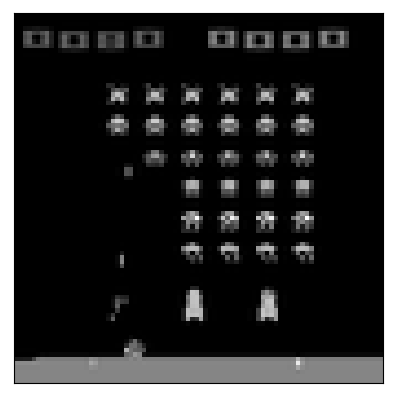
\includegraphics[scale=0.4]{figures/results/latent_image/beta_4_sample_3_reconstructed.png}
    \caption{$\beta = 4$}
\end{multicols}
\caption{A selection of Space Invader frames and their corresponding reconstructions for different values of $\beta$.}
\label{fig:latent_image_originals_and_reconstructions}
\end{figure*}


\begin{figure*}[h!]
\centering
\captionsetup{justification=centering}
\begin{multicols}{4}
    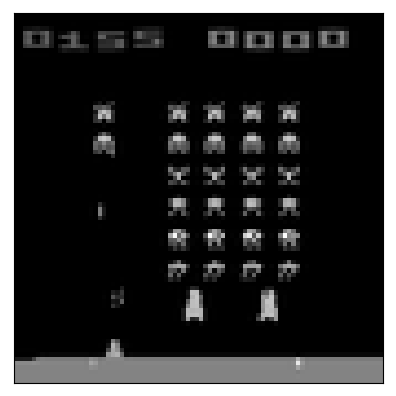
\includegraphics[scale=0.4]{figures/results/latent_image/beta_1_sample_10_original.png}
    \caption{Original}
    
\includegraphics[scale=0.4]{figures/results/latent_image/beta_1_sample_10_latent.png}
    \caption{$\beta=1$}
    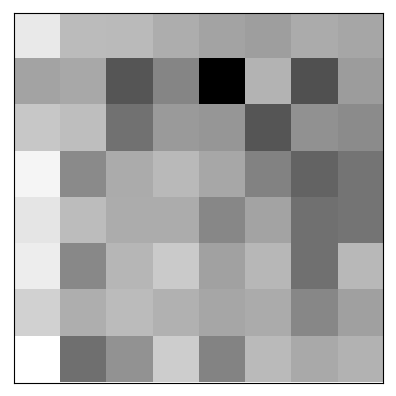
\includegraphics[scale=0.4]{figures/results/latent_image/beta_2_sample_10_latent.png}
    \caption{$\beta=2$}
    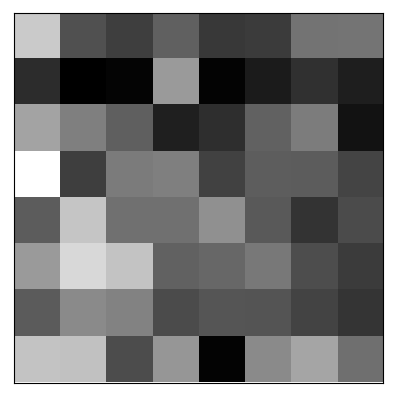
\includegraphics[scale=0.4]{figures/results/latent_image/beta_4_sample_10_latent.png}
    \caption{$\beta=4$}
\end{multicols}
\begin{multicols}{4}
    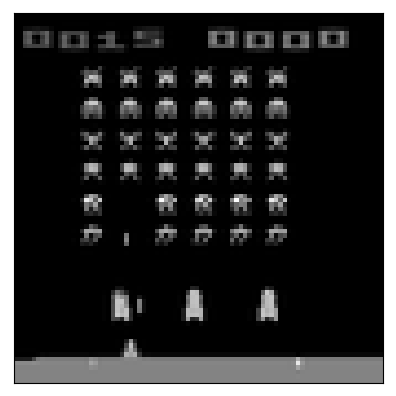
\includegraphics[scale=0.4]{figures/results/latent_image/beta_1_sample_30_original.png}
    \caption{Original}
    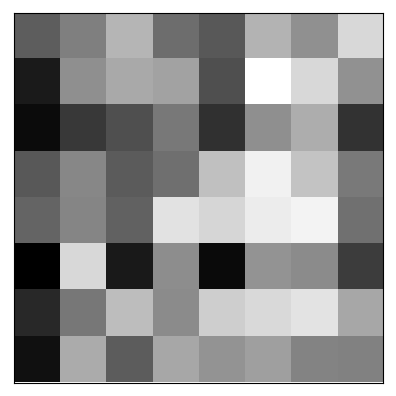
\includegraphics[scale=0.4]{figures/results/latent_image/beta_1_sample_30_latent.png}
    \caption{$\beta=1$}
    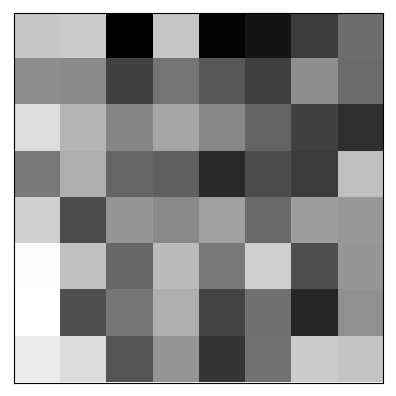
\includegraphics[scale=0.4]{figures/results/latent_image/beta_2_sample_30_latent.png}
    \caption{$\beta=2$}
    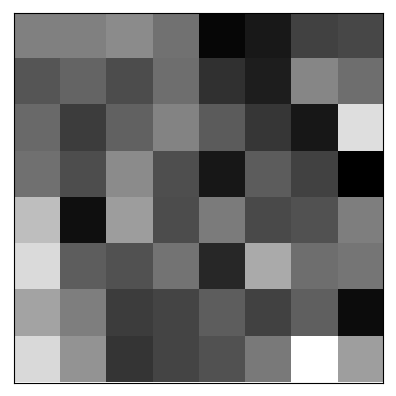
\includegraphics[scale=0.4]{figures/results/latent_image/beta_4_sample_30_latent.png}
    \caption{$\beta=4$}
\end{multicols}
\begin{multicols}{4}
    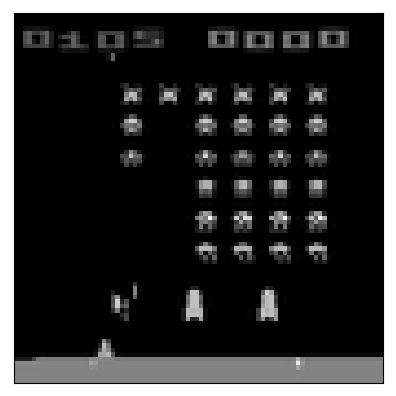
\includegraphics[scale=0.4]{figures/results/latent_image/beta_1_sample_90_original.png}
    \caption{Original}
    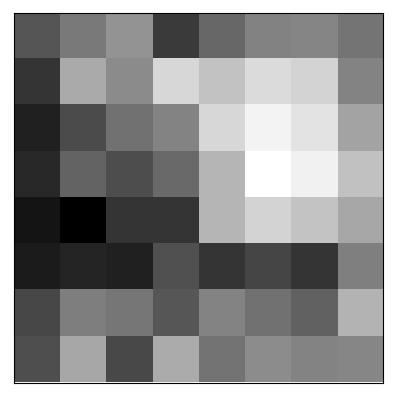
\includegraphics[scale=0.4]{figures/results/latent_image/beta_1_sample_90_latent.png}
    \caption{$\beta=1$}
    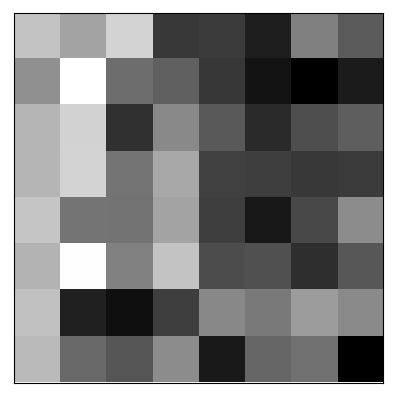
\includegraphics[scale=0.4]{figures/results/latent_image/beta_2_sample_90_latent.png}
    \caption{$\beta=2$}
    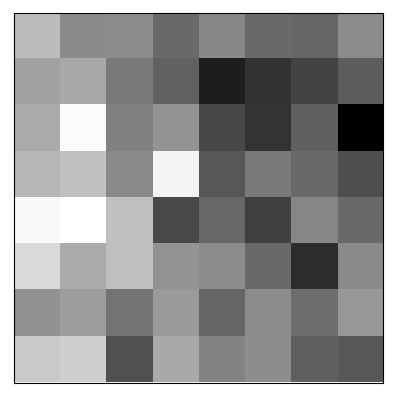
\includegraphics[scale=0.4]{figures/results/latent_image/beta_4_sample_90_latent.png}
    \caption{$\beta=4$}
\end{multicols}
\caption{Frames from Space Invaders and their corresponding latent images for different values of $\beta$.}
\label{fig:latent_image_originals_and_latent_spaces}
\end{figure*}


\begin{figure*}[h!]
\centering
\captionsetup{justification=centering}
\begin{multicols}{3}
    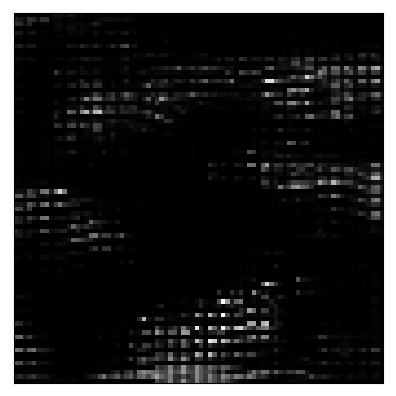
\includegraphics[scale=0.4]{figures/results/latent_image/beta_1_prior_sample_1.png}
    \caption{$\beta=1$}
    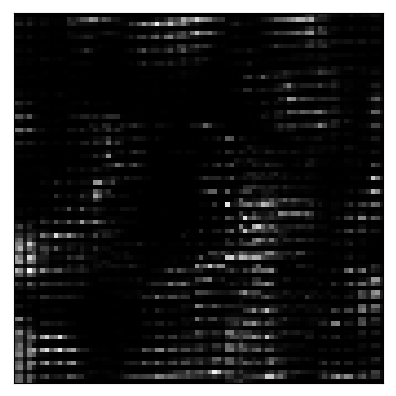
\includegraphics[scale=0.4]{figures/results/latent_image/beta_2_prior_sample_2.png}
    \caption{$\beta=2$}
    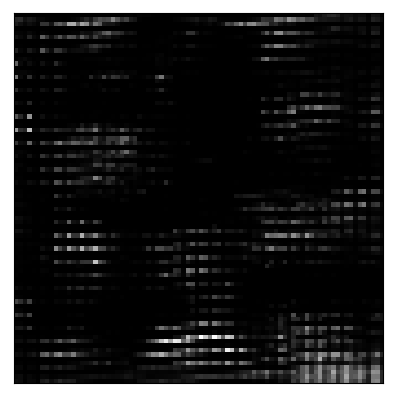
\includegraphics[scale=0.4]{figures/results/latent_image/beta_4_prior_sample_3.png}
    \caption{$\beta=4$}
\end{multicols}
\caption{The best of $10$ samples from the prior $p(\vec{z}) = \mathcal{N}(\vec{0}, \vec{I})$ for different values of $\beta$.}
\label{fig:latent_image_originals_prior_samples}
\end{figure*}


\begin{figure*}[h!]
\centering
\captionsetup{justification=centering}
\begin{multicols}{4}
    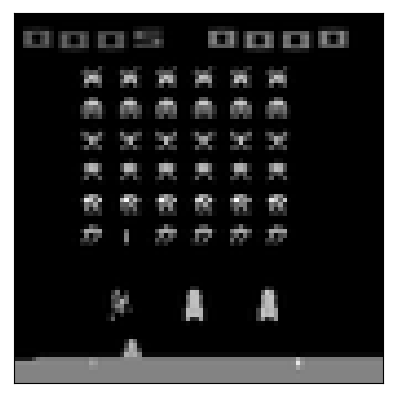
\includegraphics[scale=0.4]{figures/results/latent_image/beta_1_posterior_sample_original.png}
    \caption{Original}
    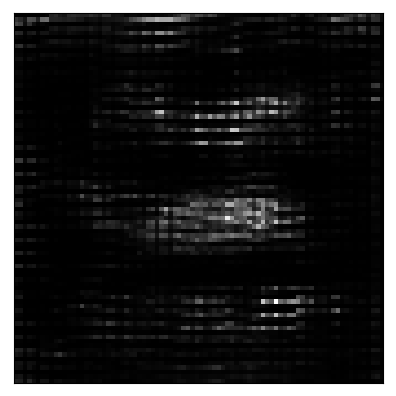
\includegraphics[scale=0.4]{figures/results/latent_image/beta_1_posterior_sample_0.png}
    \caption{$\beta=1$}
    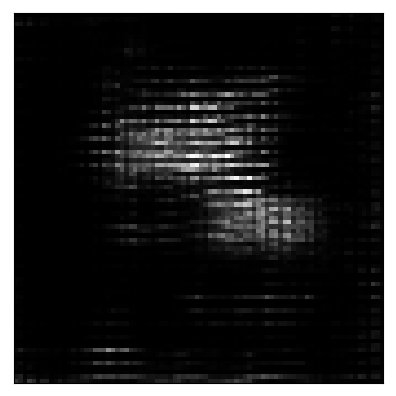
\includegraphics[scale=0.4]{figures/results/latent_image/beta_2_posterior_sample_0.png}
    \caption{$\beta=2$}
    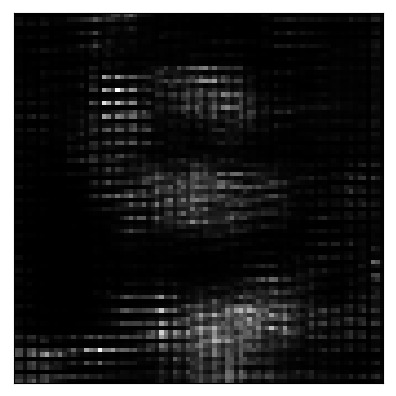
\includegraphics[scale=0.4]{figures/results/latent_image/beta_4_posterior_sample_0.png}
    \caption{$\beta=4$}
\end{multicols}
\caption{Samples from posterior after one step of MCMC for different values of $\beta$. Samples for subsequent steps did not improve, hence we only include the first for each value of $\beta$.}
\label{fig:latent_image_originals_posterior_samples}
\end{figure*}


\begin{figure*}[h!]
\centering
\captionsetup{justification=centering}
\begin{multicols}{3}
    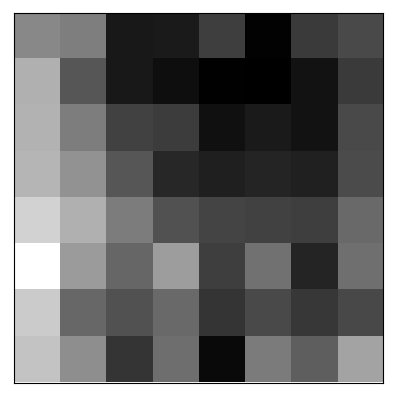
\includegraphics[scale=0.4]{figures/results/latent_image/beta_1_average_activation.png}
    \caption{$\beta=1$}
    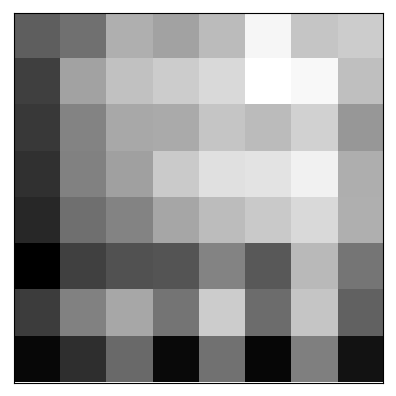
\includegraphics[scale=0.4]{figures/results/latent_image/beta_2_average_activation.png}
    \caption{$\beta=2$}
    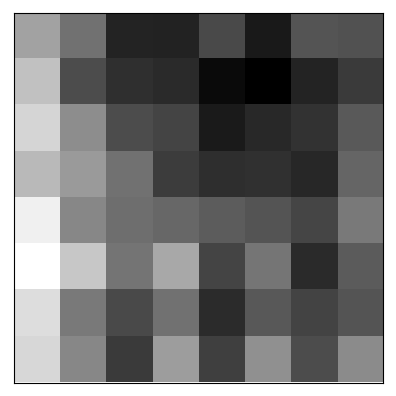
\includegraphics[scale=0.4]{figures/results/latent_image/beta_4_average_activation.png}
    \caption{$\beta=4$}
\end{multicols}
\caption{An average of the activations in the latent image over $10000$ images from the test set for different values of $\beta$.}
\label{fig:latent_image_originals_posterior_samples}
\end{figure*}

%
%
%
%
%
\section{Disentangling Latent Neurons}
\begin{itemize}
\item Consider two architectures: shallow and deep
\item Consider Pong, Space Invaders (in progress) and Breakout
\item Plot reconstruction loss and KL divergence
\item Show reconstructions and convolutional layers of each
\item Show mean activations of filters
\item Alter latent space variable and show reconstruction
\item Add noise to filters
\end{itemize}



\begin{figure*}[h!]
\centering
\captionsetup{justification=centering}
    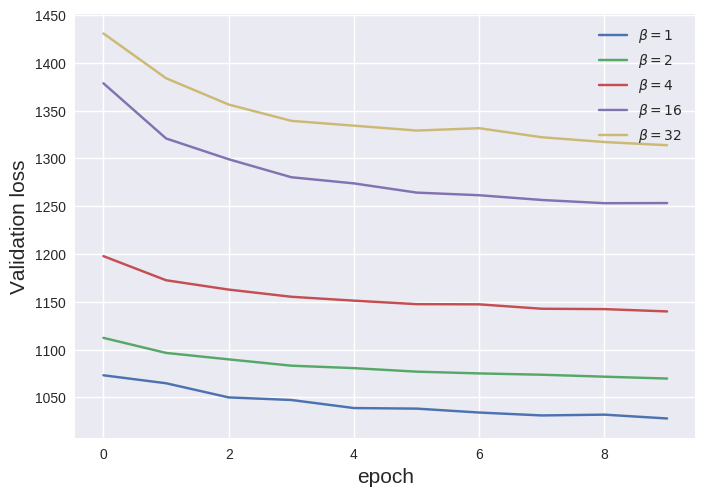
\includegraphics[scale=0.5]{figures/results/indiscriminate_decoupling/val_loss.png}
    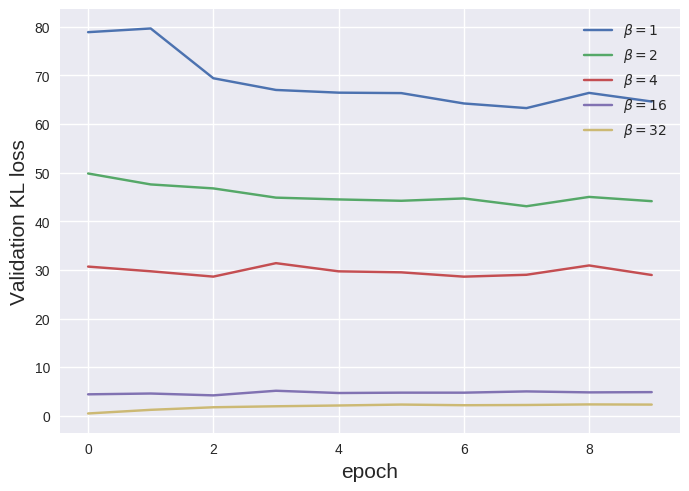
\includegraphics[scale=0.5]{figures/results/indiscriminate_decoupling/val_kl_loss.png}
    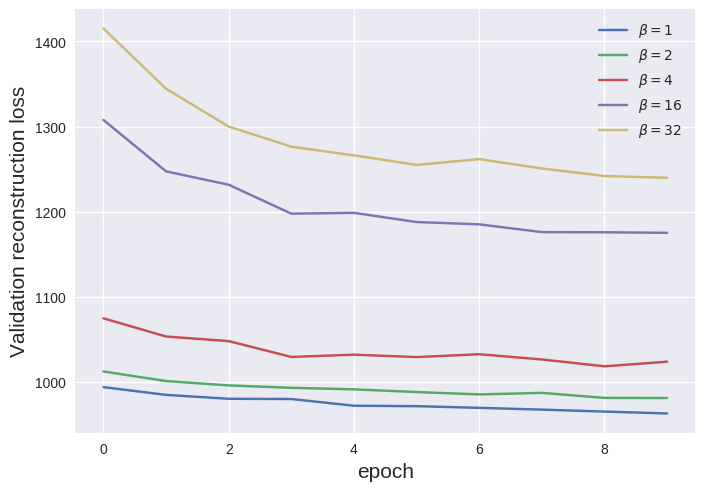
\includegraphics[scale=0.5]{figures/results/indiscriminate_decoupling/val_reconstruction_loss.png}
\caption{Disentangling latent neurons.}
\label{fig:indiscriminate_decoupling_graphs}
\end{figure*}



\begin{figure*}[h!]
\centering
\captionsetup{justification=centering}
\begin{multicols}{4}
    \includegraphics[scale=0.4]{figures/results/indiscriminate_decoupling/beta_1_sample_0_original.png}
    \caption{Original}
    \includegraphics[scale=0.4]{figures/results/indiscriminate_decoupling/beta_1_sample_0_reconstructed.png}
    \caption{$\beta = 1$}    
    \includegraphics[scale=0.4]{figures/results/indiscriminate_decoupling/beta_2_sample_0_reconstructed.png}
    \caption{$\beta = 2$}
    \includegraphics[scale=0.4]{figures/results/indiscriminate_decoupling/beta_4_sample_0_reconstructed.png}
    \caption{$\beta = 4$}
\end{multicols}
\begin{multicols}{4}
    \includegraphics[scale=0.4]{figures/results/indiscriminate_decoupling/beta_1_sample_2_original.png}
    \caption{Original}
    \includegraphics[scale=0.4]{figures/results/indiscriminate_decoupling/beta_1_sample_2_reconstructed.png}
    \caption{$\beta = 1$}    
    \includegraphics[scale=0.4]{figures/results/indiscriminate_decoupling/beta_2_sample_2_reconstructed.png}
    \caption{$\beta = 2$}
    \includegraphics[scale=0.4]{figures/results/indiscriminate_decoupling/beta_4_sample_2_reconstructed.png}
    \caption{$\beta = 4$}
\end{multicols}
\begin{multicols}{4}
    \includegraphics[scale=0.4]{figures/results/indiscriminate_decoupling/beta_1_sample_3_original.png}
    \caption{Original}
    \includegraphics[scale=0.4]{figures/results/indiscriminate_decoupling/beta_1_sample_3_reconstructed.png}
    \caption{$\beta = 1$}
    \includegraphics[scale=0.4]{figures/results/indiscriminate_decoupling/beta_2_sample_3_reconstructed.png}
    \caption{$\beta = 2$}
    \includegraphics[scale=0.4]{figures/results/indiscriminate_decoupling/beta_4_sample_3_reconstructed.png}
    \caption{$\beta = 4$}
\end{multicols}
\caption{A selection of Space Invader frames and their corresponding reconstructions for different values of $\beta$.}
\label{fig:indiscriminate_decoupling_originals_and_reconstructions}
\end{figure*}


\begin{figure*}[h!]
\centering
\captionsetup{justification=centering}
\begin{minipage}{0.4\textwidth}
\centering
\captionsetup{justification=centering}
\includegraphics[scale=0.4]{figures/results/indiscriminate_decoupling/beta_1_sample_3_original.png}
\caption{Original}
\end{minipage}
\begin{minipage}{0.55\textwidth}
\centering
\captionsetup{justification=centering}
\includegraphics[scale=0.42]{figures/results/indiscriminate_decoupling/beta_1_convolutional_layers_sample_3.png}
\caption{$\beta = 1$}
\includegraphics[scale=0.42]{figures/results/indiscriminate_decoupling/beta_2_convolutional_layers_sample_3.png}
\caption{$\beta = 2$}
\includegraphics[scale=0.42]{figures/results/indiscriminate_decoupling/beta_4_convolutional_layers_sample_3.png}
\caption{$\beta = 4$}
\end{minipage}
\caption{A Space Invaders frame and the activations over its corresponding latent filters for different values of $\beta$.}
\label{fig:indiscriminate_decoupling_originals_and_latent_filters}
\end{figure*}


\begin{figure*}[h!]
\centering
\captionsetup{justification=centering}
\begin{multicols}{3}
    \includegraphics[scale=0.4]{figures/results/indiscriminate_decoupling/beta_1_prior_sample_2.png}
    \caption{$\beta=1$}
    \includegraphics[scale=0.4]{figures/results/indiscriminate_decoupling/beta_2_prior_sample_0.png}
    \caption{$\beta=2$}
    \includegraphics[scale=0.4]{figures/results/indiscriminate_decoupling/beta_4_prior_sample_3.png}
    \caption{$\beta=4$}
\end{multicols}
\caption{The best of $10$ samples from the prior $p(\vec{z}) = \mathcal{N}(\vec{0}, \vec{I})$ for different values of $\beta$.}
\label{fig:indiscriminate_decoupling_prior_samples}
\end{figure*}


\begin{figure*}[h!]
\centering
\captionsetup{justification=centering}
\begin{multicols}{4}
    \includegraphics[scale=0.4]{figures/results/indiscriminate_decoupling/beta_1_posterior_sample_original.png}
    \caption{$\beta=1\quad$ (original)}
    \includegraphics[scale=0.4]{figures/results/indiscriminate_decoupling/beta_1_posterior_sample_10.png}
    \caption{$\beta=1\quad$ (19 steps)}
    \includegraphics[scale=0.4]{figures/results/indiscriminate_decoupling/beta_1_posterior_sample_26.png}
    \caption{$\beta=1\quad$ (26 steps)}
    \includegraphics[scale=0.4]{figures/results/indiscriminate_decoupling/beta_1_posterior_sample_60.png}
    \caption{$\beta=1\quad$ (60 steps)}
\end{multicols}

\begin{multicols}{4}
    \includegraphics[scale=0.4]{figures/results/indiscriminate_decoupling/beta_2_posterior_sample_original.png}
    \caption{$\beta=2\quad$ (original)}
    \includegraphics[scale=0.4]{figures/results/indiscriminate_decoupling/beta_2_posterior_sample_0.png}
    \caption{$\beta=2\quad$ (1 step)}
    \includegraphics[scale=0.4]{figures/results/indiscriminate_decoupling/beta_2_posterior_sample_1.png}
    \caption{$\beta=2\quad$ (2 steps)}
    \includegraphics[scale=0.4]{figures/results/indiscriminate_decoupling/beta_2_posterior_sample_90.png}
    \caption{$\beta=2\quad$ (90 steps)}
\end{multicols}

\begin{multicols}{4}
    \includegraphics[scale=0.4]{figures/results/indiscriminate_decoupling/beta_4_posterior_sample_original.png}
    \caption{$\beta=4\quad$ (original)}
    \includegraphics[scale=0.4]{figures/results/indiscriminate_decoupling/beta_4_posterior_sample_0.png}
    \caption{$\beta=4\quad$ (1 step)}
    \includegraphics[scale=0.4]{figures/results/indiscriminate_decoupling/beta_4_posterior_sample_7.png}
    \caption{$\beta=4\quad$ (7 steps)}
    \includegraphics[scale=0.4]{figures/results/indiscriminate_decoupling/beta_4_posterior_sample_98.png}
    \caption{$\beta=4\quad$ (98 steps)}
\end{multicols}

\caption{An average of the activations in the latent image over $10000$ images from the test set for different values of $\beta$.}
\label{fig:indiscriminate_decoupling_posterior_samples}
\end{figure*}


\begin{figure*}[h!]
\centering
\captionsetup{justification=centering}

    \includegraphics[scale=0.3]{figures/results/indiscriminate_decoupling/beta_1_average_activation.png}
    \caption{$\beta=1$}
    \includegraphics[scale=0.3]{figures/results/indiscriminate_decoupling/beta_2_average_activation.png}
    \caption{$\beta=2$}
    \includegraphics[scale=0.3]{figures/results/indiscriminate_decoupling/beta_4_average_activation.png}
    \caption{$\beta=4$}

\caption{An average of the activations in the latent image over $10000$ images from the test set for different values of $\beta$.}
\label{fig:indiscriminate_decoupling_originals_posterior_samples}
\end{figure*}





%
%
%
%
%
\section{Disentangling Latent Filters Using Averages}
\begin{itemize}
\item Consider two architectures: shallow and deep
\item Consider Pong, Space Invaders (done) and Breakout
\item Plot reconstruction loss and KL divergence
\item Show reconstructions and convolutional layers of each
\item Show mean activations of filters
\item Alter latent space variable and show reconstruction
\item Add noise to filters
\end{itemize}


\begin{figure*}[h!]
\centering
\captionsetup{justification=centering}
    \includegraphics[scale=0.5]{figures/results/naive_average/val_loss.png}
    \includegraphics[scale=0.5]{figures/results/naive_average/val_kl_loss.png}
    \includegraphics[scale=0.5]{figures/results/naive_average/val_reconstruction_loss.png}
\caption{Naive average.}
\label{fig:naive_average_graphs}
\end{figure*}


\begin{figure*}[h!]
\centering
\captionsetup{justification=centering}
\begin{multicols}{4}
    \includegraphics[scale=0.4]{figures/results/naive_average/beta_1_sample_0_original.png}
    \caption{Original}
    \includegraphics[scale=0.4]{figures/results/naive_average/beta_1_sample_0_reconstructed.png}
    \caption{$\beta = 1$}    
    \includegraphics[scale=0.4]{figures/results/naive_average/beta_2_sample_0_reconstructed.png}
    \caption{$\beta = 2$}
    \includegraphics[scale=0.4]{figures/results/naive_average/beta_4_sample_0_reconstructed.png}
    \caption{$\beta = 4$}
\end{multicols}
\begin{multicols}{4}
    \includegraphics[scale=0.4]{figures/results/naive_average/beta_1_sample_2_original.png}
    \caption{Original}
    \includegraphics[scale=0.4]{figures/results/naive_average/beta_1_sample_2_reconstructed.png}
    \caption{$\beta = 1$}    
    \includegraphics[scale=0.4]{figures/results/naive_average/beta_2_sample_2_reconstructed.png}
    \caption{$\beta = 2$}
    \includegraphics[scale=0.4]{figures/results/naive_average/beta_4_sample_2_reconstructed.png}
    \caption{$\beta = 4$}
\end{multicols}
\begin{multicols}{4}
    \includegraphics[scale=0.4]{figures/results/naive_average/beta_1_sample_3_original.png}
    \caption{Original}
    \includegraphics[scale=0.4]{figures/results/naive_average/beta_1_sample_3_reconstructed.png}
    \caption{$\beta = 1$}
    \includegraphics[scale=0.4]{figures/results/naive_average/beta_2_sample_3_reconstructed.png}
    \caption{$\beta = 2$}
    \includegraphics[scale=0.4]{figures/results/naive_average/beta_4_sample_3_reconstructed.png}
    \caption{$\beta = 4$}
\end{multicols}
\caption{A selection of Space Invader frames and their corresponding reconstructions for different values of $\beta$.}
\label{fig:naive_average_originals_and_reconstructions}
\end{figure*}



\begin{figure*}[h!]
\centering
\captionsetup{justification=centering}
\begin{minipage}{0.4\textwidth}
\centering
\captionsetup{justification=centering}
\includegraphics[scale=0.4]{figures/results/naive_average/beta_1_sample_3_original.png}
\caption{Original}
\end{minipage}
\begin{minipage}{0.55\textwidth}
\centering
\captionsetup{justification=centering}
\includegraphics[scale=0.42]{figures/results/naive_average/beta_1_convolutional_layers_sample_3.png}
\caption{$\beta = 1$}
\includegraphics[scale=0.42]{figures/results/naive_average/beta_2_convolutional_layers_sample_3.png}
\caption{$\beta = 2$}
\includegraphics[scale=0.42]{figures/results/naive_average/beta_4_convolutional_layers_sample_3.png}
\caption{$\beta = 4$}
\end{minipage}
\caption{A Space Invaders frame and the activations over its corresponding latent filters for different values of $\beta$.}
\label{fig:naive_average_originals_and_latent_filters}
\end{figure*}



\begin{figure*}[h!]
\centering
\captionsetup{justification=centering}
\begin{multicols}{3}
    \includegraphics[scale=0.4]{figures/results/naive_average/beta_1_prior_sample_2.png}
    \caption{$\beta=1$}
    \includegraphics[scale=0.4]{figures/results/naive_average/beta_2_prior_sample_0.png}
    \caption{$\beta=2$}
    \includegraphics[scale=0.4]{figures/results/naive_average/beta_4_prior_sample_3.png}
    \caption{$\beta=4$}
\end{multicols}
\caption{The best of $10$ samples from the prior $p(\vec{z}) = \mathcal{N}(\vec{0}, \vec{I})$ for different values of $\beta$.}
\label{fig:naive_average_decoupling_prior_samples}
\end{figure*}


\begin{figure*}[h!]
\centering
\captionsetup{justification=centering}
\begin{multicols}{4}
    \includegraphics[scale=0.4]{figures/results/naive_average/beta_1_posterior_sample_original.png}
    \caption{Original}
    \includegraphics[scale=0.4]{figures/results/naive_average/beta_1_posterior_sample_0.png}
    \caption{$\beta=1$}
    \includegraphics[scale=0.4]{figures/results/naive_average/beta_2_posterior_sample_0.png}
    \caption{$\beta=2$}
    \includegraphics[scale=0.4]{figures/results/naive_average/beta_4_posterior_sample_0.png}
    \caption{$\beta=4$}
\end{multicols}
\caption{Samples from posterior after one step of MCMC for different values of $\beta$. Samples for subsequent steps did not improve, hence we only include the first for each value of $\beta$.}
\label{fig:naive_average_originals_posterior_samples}
\end{figure*}



\begin{figure*}[h!]
\centering
\captionsetup{justification=centering}

    \includegraphics[scale=0.3]{figures/results/naive_average/beta_1_average_activation.png}
    \caption{$\beta=1$}
    \includegraphics[scale=0.3]{figures/results/naive_average/beta_2_average_activation.png}
    \caption{$\beta=2$}
    \includegraphics[scale=0.3]{figures/results/naive_average/beta_4_average_activation.png}
    \caption{$\beta=4$}

\caption{An average of the activations in the latent image over $10000$ images from the test set for different values of $\beta$.}
\label{fig:naive_average_originals_posterior_samples}
\end{figure*}



%
%
%
%
%
\section{Decoupling Latent Filters Using Weighted-Averages}
\begin{itemize}
\item Consider two architectures: shallow and deep
\item Consider Pong, Space Invaders (done) and Breakout
\item Plot reconstruction loss and KL divergence
\item Show reconstructions and convolutional layers of each
\item Show mean activations of filters
\item Alter latent space variable and show reconstruction
\item Add noise to filters
\end{itemize}



\begin{figure*}[h!]
\centering
\captionsetup{justification=centering}
    \includegraphics[scale=0.5]{figures/results/weighted_average/val_loss.png}
    \includegraphics[scale=0.5]{figures/results/weighted_average/val_kl_loss.png}
    \includegraphics[scale=0.5]{figures/results/weighted_average/val_reconstruction_loss.png}
\caption{Caption.}
\label{fig:weighted_average_graphs}
\end{figure*}




\begin{figure*}[h!]
\centering
\captionsetup{justification=centering}
\begin{multicols}{4}
    \includegraphics[scale=0.4]{figures/results/weighted_average/beta_1_sample_0_original.png}
    \caption{Original}
    \includegraphics[scale=0.4]{figures/results/weighted_average/beta_1_sample_0_reconstructed.png}
    \caption{$\beta = 1$}    
    \includegraphics[scale=0.4]{figures/results/weighted_average/beta_2_sample_0_reconstructed.png}
    \caption{$\beta = 2$}
    \includegraphics[scale=0.4]{figures/results/weighted_average/beta_4_sample_0_reconstructed.png}
    \caption{$\beta = 4$}
\end{multicols}
\begin{multicols}{4}
    \includegraphics[scale=0.4]{figures/results/weighted_average/beta_1_sample_2_original.png}
    \caption{Original}
    \includegraphics[scale=0.4]{figures/results/weighted_average/beta_1_sample_2_reconstructed.png}
    \caption{$\beta = 1$}    
    \includegraphics[scale=0.4]{figures/results/weighted_average/beta_2_sample_2_reconstructed.png}
    \caption{$\beta = 2$}
    \includegraphics[scale=0.4]{figures/results/weighted_average/beta_4_sample_2_reconstructed.png}
    \caption{$\beta = 4$}
\end{multicols}
\begin{multicols}{4}
    \includegraphics[scale=0.4]{figures/results/weighted_average/beta_1_sample_3_original.png}
    \caption{Original}
    \includegraphics[scale=0.4]{figures/results/weighted_average/beta_1_sample_3_reconstructed.png}
    \caption{$\beta = 1$}
    \includegraphics[scale=0.4]{figures/results/weighted_average/beta_2_sample_3_reconstructed.png}
    \caption{$\beta = 2$}
    \includegraphics[scale=0.4]{figures/results/weighted_average/beta_4_sample_3_reconstructed.png}
    \caption{$\beta = 4$}
\end{multicols}
\caption{A selection of Space Invader frames and their corresponding reconstructions for different values of $\beta$.}
\label{fig:weighted_average_originals_and_reconstructions}
\end{figure*}




\begin{figure*}[h!]
\centering
\captionsetup{justification=centering}
\begin{minipage}{0.4\textwidth}
\centering
\captionsetup{justification=centering}
\includegraphics[scale=0.4]{figures/results/weighted_average/beta_1_sample_3_original.png}
\caption{Original}
\end{minipage}
\begin{minipage}{0.55\textwidth}
\centering
\captionsetup{justification=centering}
\includegraphics[scale=0.42]{figures/results/weighted_average/beta_1_convolutional_layers_sample_3.png}
\caption{$\beta = 1$}
\includegraphics[scale=0.42]{figures/results/weighted_average/beta_2_convolutional_layers_sample_3.png}
\caption{$\beta = 2$}
\includegraphics[scale=0.42]{figures/results/weighted_average/beta_4_convolutional_layers_sample_3.png}
\caption{$\beta = 4$}
\end{minipage}
\caption{A Space Invaders frame and the activations over its corresponding latent filters for different values of $\beta$.}
\label{fig:weighted_average_originals_and_latent_filters}
\end{figure*}

\begin{itemize}
\item Sampling from prior makes no sense (explained earlier)
\item We observe the same result, which wont be included
\end{itemize}



\begin{figure*}[h!]
\centering
\captionsetup{justification=centering}
\begin{multicols}{4}
    \includegraphics[scale=0.4]{figures/results/weighted_average/beta_1_posterior_sample_original.png}
    \caption{$\beta=1\quad$ (original)}
    \includegraphics[scale=0.4]{figures/results/weighted_average/beta_1_posterior_sample_18.png}
    \caption{$\beta=1\quad$ (18 steps)}
    \includegraphics[scale=0.4]{figures/results/weighted_average/beta_1_posterior_sample_26.png}
    \caption{$\beta=1\quad$ (26 steps)}
    \includegraphics[scale=0.4]{figures/results/weighted_average/beta_1_posterior_sample_39.png}
    \caption{$\beta=1\quad$ (39 steps)}
\end{multicols}

\begin{multicols}{4}
    \includegraphics[scale=0.4]{figures/results/weighted_average/beta_2_posterior_sample_original.png}
    \caption{$\beta=2\quad$ (original)}
    \includegraphics[scale=0.4]{figures/results/weighted_average/beta_2_posterior_sample_17.png}
    \caption{$\beta=2\quad$ (17 steps)}
    \includegraphics[scale=0.4]{figures/results/weighted_average/beta_2_posterior_sample_26.png}
    \caption{$\beta=2\quad$ (26 steps)}
    \includegraphics[scale=0.4]{figures/results/weighted_average/beta_2_posterior_sample_30.png}
    \caption{$\beta=2\quad$ (30 steps)}
\end{multicols}

\begin{multicols}{4}
    \includegraphics[scale=0.4]{figures/results/weighted_average/beta_4_posterior_sample_original.png}
    \caption{$\beta=4\quad$ (original)}
    \includegraphics[scale=0.4]{figures/results/weighted_average/beta_4_posterior_sample_7.png}
    \caption{$\beta=4\quad$ (7 steps)}
    \includegraphics[scale=0.4]{figures/results/weighted_average/beta_4_posterior_sample_24.png}
    \caption{$\beta=4\quad$ (24 steps)}
    \includegraphics[scale=0.4]{figures/results/weighted_average/beta_4_posterior_sample_32.png}
    \caption{$\beta=4\quad$ (32 steps)}
\end{multicols}

\caption{An average of the activations in the latent image over $10,000$ images from the test set for different values of $\beta$.}
\label{fig:weighted_average_posterior_samples}
\end{figure*}



\begin{figure*}[h!]
\centering
\captionsetup{justification=centering}

    \includegraphics[scale=0.42]{figures/results/weighted_average/beta_1_average_activation.png}
    \caption{$\beta=1$}
    \includegraphics[scale=0.42]{figures/results/weighted_average/beta_2_average_activation.png}
    \caption{$\beta=2$}
    \includegraphics[scale=0.42]{figures/results/weighted_average/beta_4_average_activation.png}
    \caption{$\beta=4$}

\caption{An average of the activations in the latent image over $10,000$ images from the test set for different values of $\beta$.}
\label{fig:weighted_average_originals_posterior_samples}
\end{figure*}



%
%
%
%
%
\section{Separating Colour Spaces}
\begin{itemize}
\item Consider two architectures: shallow and deep
\item Consider Pong, Space Invaders (in progress) and Breakout
\item Plot reconstruction loss and KL divergence
\item Show reconstructions and convolutional layers of each
\item Show mean activations of filters
\item Alter latent space variable and show reconstruction
\item Add noise to filters
\end{itemize}




\begin{figure*}[h!]
\centering
\captionsetup{justification=centering}
\begin{multicols}{4}
    \includegraphics[scale=0.4]{figures/results/colour_separated/beta_1_sample_0_original.png}
    \caption{Original}
    \includegraphics[scale=0.4]{figures/results/colour_separated/beta_1_sample_0_reconstructed.png}
    \caption{$\beta = 1$}    
    \includegraphics[scale=0.4]{figures/results/colour_separated/beta_2_sample_0_reconstructed.png}
    \caption{$\beta = 2$}
    \includegraphics[scale=0.4]{figures/results/colour_separated/beta_4_sample_0_reconstructed.png}
    \caption{$\beta = 4$}
\end{multicols}
\begin{multicols}{4}
    \includegraphics[scale=0.4]{figures/results/colour_separated/beta_1_sample_2_original.png}
    \caption{Original}
    \includegraphics[scale=0.4]{figures/results/colour_separated/beta_1_sample_2_reconstructed.png}
    \caption{$\beta = 1$}    
    \includegraphics[scale=0.4]{figures/results/colour_separated/beta_2_sample_2_reconstructed.png}
    \caption{$\beta = 2$}
    \includegraphics[scale=0.4]{figures/results/colour_separated/beta_4_sample_2_reconstructed.png}
    \caption{$\beta = 4$}
\end{multicols}
\begin{multicols}{4}
    \includegraphics[scale=0.4]{figures/results/colour_separated/beta_1_sample_3_original.png}
    \caption{Original}
    \includegraphics[scale=0.4]{figures/results/colour_separated/beta_1_sample_3_reconstructed.png}
    \caption{$\beta = 1$}    
    \includegraphics[scale=0.4]{figures/results/colour_separated/beta_2_sample_3_reconstructed.png}
    \caption{$\beta = 2$}
    \includegraphics[scale=0.4]{figures/results/colour_separated/beta_4_sample_3_reconstructed.png}
    \caption{$\beta = 4$}
\end{multicols}
\caption{A selection of Space Invader frames and their corresponding reconstructions for different values of $\beta$.}
\label{fig:colour_separated_originals_and_reconstructions}
\end{figure*}



\begin{figure*}[h!]
\centering
\captionsetup{justification=centering}
\begin{minipage}{0.4\textwidth}
\centering
\captionsetup{justification=centering}
\includegraphics[scale=0.4]{figures/results/colour_separated/beta_1_sample_3_original.png}
\caption{Original}
\end{minipage}
\begin{minipage}{0.55\textwidth}
\centering
\captionsetup{justification=centering}
\includegraphics[scale=0.42]{figures/results/colour_separated/beta_1_convolutional_layers_sample_3.png}
\caption{$\beta = 1$}
\includegraphics[scale=0.42]{figures/results/colour_separated/beta_2_convolutional_layers_sample_3.png}
\caption{$\beta = 2$}
\includegraphics[scale=0.42]{figures/results/colour_separated/beta_4_convolutional_layers_sample_3.png}
\caption{$\beta = 4$}
\end{minipage}
\caption{A Space Invaders frame and the activations over its corresponding latent filters for different values of $\beta$.}
\label{fig:colour_separated_originals_and_latent_filters}
\end{figure*}






\begin{figure*}[h!]
\centering
\captionsetup{justification=centering}
\begin{multicols}{4}
    \includegraphics[scale=0.4]{figures/results/colour_separated/beta_1_posterior_sample_original.png}
    \caption{$\beta=1\quad$ (original)}
    \includegraphics[scale=0.4]{figures/results/colour_separated/beta_1_posterior_sample_7.png}
    \caption{$\beta=1\quad$ (7 steps)}
    \includegraphics[scale=0.4]{figures/results/colour_separated/beta_1_posterior_sample_13.png}
    \caption{$\beta=1\quad$ (17 steps)}
    \includegraphics[scale=0.4]{figures/results/colour_separated/beta_1_posterior_sample_18.png}
    \caption{$\beta=1\quad$ (18 steps)}
\end{multicols}

\begin{multicols}{4}
    \includegraphics[scale=0.4]{figures/results/colour_separated/beta_2_posterior_sample_original.png}
    \caption{$\beta=2\quad$ (original)}
    \includegraphics[scale=0.4]{figures/results/colour_separated/beta_2_posterior_sample_10.png}
    \caption{$\beta=2\quad$ (10 steps)}
    \includegraphics[scale=0.4]{figures/results/colour_separated/beta_2_posterior_sample_17.png}
    \caption{$\beta=2\quad$ (17 steps)}
    \includegraphics[scale=0.4]{figures/results/colour_separated/beta_2_posterior_sample_31.png}
    \caption{$\beta=2\quad$ (31 steps)}
\end{multicols}

\begin{multicols}{4}
    \includegraphics[scale=0.4]{figures/results/colour_separated/beta_4_posterior_sample_original.png}
    \caption{$\beta=4\quad$ (original)}
    \includegraphics[scale=0.4]{figures/results/colour_separated/beta_4_posterior_sample_1.png}
    \caption{$\beta=4\quad$ (1 step)}
    \includegraphics[scale=0.4]{figures/results/colour_separated/beta_4_posterior_sample_4.png}
    \caption{$\beta=4\quad$ (3 steps)}
    \includegraphics[scale=0.4]{figures/results/colour_separated/beta_4_posterior_sample_20.png}
    \caption{$\beta=4\quad$ (20 steps)}
\end{multicols}

\caption{An average of the activations in the latent image over $10,000$ images from the test set for different values of $\beta$.}
\label{fig:weighted_average_posterior_samples}
\end{figure*}


\begin{figure*}[h!]
\centering
\captionsetup{justification=centering}

    \includegraphics[scale=0.42]{figures/results/colour_separated/beta_1_average_activation.png}
    \caption{$\beta=1$}
    \includegraphics[scale=0.42]{figures/results/colour_separated/beta_2_average_activation.png}
    \caption{$\beta=2$}
    \includegraphics[scale=0.42]{figures/results/colour_separated/beta_4_average_activation.png}
    \caption{$\beta=4$}

\caption{An average of the activations in the latent image over $10,000$ images from the test set for different values of $\beta$.}
\label{fig:weighted_average_originals_posterior_samples}
\end{figure*}


%
%
%
%
%
\section{Orthogonal Convolutions}
\begin{itemize}
\item Consider two architectures: shallow and deep
\item Consider Pong, Space Invaders and Breakout
\item Plot reconstruction loss and KL divergence
\item Show reconstructions and convolutional layers of each
\item Alter latent space variable and show reconstruction
\item Add noise to filters
\end{itemize}



%
%
%
%
%
\section{Winner Takes All}
\begin{itemize}
\item Consider two architectures: shallow and deep
\item Consider Pong, Space Invaders and Breakout
\item Plot reconstruction loss and KL divergence
\item Show reconstructions and convolutional layers of each
\item Show mean activations of filters
\item Alter latent space variable and show reconstruction
\item Show samples from prior and posterior
\item Add noise to filters
\end{itemize}


%
%
%
%
%
\section{The No Free Lunch Relationship Between Reconstruction Loss and KL Divergence}

\begin{itemize}
\item Vary $\beta$ and plot BCE and KL
\item Show example images for different $\beta$
\item Consider Space Invaders, Pong and Breakout
\end{itemize}

%
%
%
%
%
\section{Using Batch Normalisation With Convolutional Variational Latent Spaces}

\begin{itemize}
\item Consider single architecture 
\item Batch norm before, after, both, and none
\end{itemize}